\chapter{Estado del arte}

{\color{blue}

Antes de empezar a desarrollar los objetivos del proyecto es necesario conocer primero los fundamentos del Internet de las Cosas, esto engloba desde su funcionamiento, tipos de arquitecturas hasta los distintos estándares que existen.

\section{Internet de las Cosas} \label{sec:iot}

El término ``Internet de las Cosas`` (IoT) se conoce desde hace unos años. En los últimos tiempos, está recibiendo más atención debido al avance de la tecnología inalámbrica. La idea básica se debe a la variedad de objetos, como RFID, sensores, actuadores, teléfonos móviles, que pueden interactuar entre sí teniendo una dirección distinta. El IoT permite a los objetos ver, oír, pensar y realizar trabajos haciendo que `hablen` entre sí, para compartir y sincronizar información. Transforma estos objetos de convencionales a inteligentes mediante la manipulación de sus tecnologías subyacentes, como los dispositivos integrados, las tecnologías de comunicación, las redes de sensores, los protocolos y las aplicaciones. \cite{7589556} \\

La premisa básica y el objetivo de IoT es ``conectar lo que no está conectado``. Esto significa que los objetos que no están actualmente unidos a una red informática, es decir, a Internet, se conectarán para que puedan comunicarse e interactuar con personas y otros objetos. IoT es una transición tecnológica en la que los dispositivos nos permitirán sentir y controlar el mundo físico haciendo que los objetos sean más inteligentes y conectándolos a través de una red inteligente. Cuando los objetos y las máquinas pueden ser detectados y controlados a distancia a través de una red, se consigue una mayor integración entre el mundo físico y los ordenadores. Esto permite mejoras en las áreas de eficiencia, precisión, automatización y habilitación de aplicaciones avanzadas. \\

El mundo del IoT es amplio y puede resultar algo complicado al principio debido a la abundancia de componentes y protocolos que engloba. En lugar de considerar IoT como un único tecnología, es bueno verlo como un paraguas de varios conceptos, protocolos y tecnologías, todos ellos dependientes a veces de un sector concreto. Aunque la amplia gama de elementos de IoT está diseñado para crear numerosos beneficios en las áreas de productividad y automatización, al mismo al mismo tiempo, introduce nuevos retos, como la ampliación del gran número de dispositivos y de la cantidad de datos que deben procesarse. \cite{hanes2017iot}

\subsection{Arquitecturas}

En esta sección se muestran distintas arquitecturas para el IoT, que suele describirse como un proceso de cuatro etapas en el que los datos fluyen desde los sensores conectados a las "cosas" a través de una red y, finalmente, a un centro de datos corporativo o a la nube para su procesamiento, análisis y almacenamiento.

\subsubsection{Arquitectura de tres capas}

Normalmente, la arquitectura de IoT se divide en tres capas básicas: capa de aplicación, capa de red y capa de percepción, que se describen con más detalle a continuación.

\begin{itemize}
    \item \textbf{Capa de percepción.} También conocida como capa de sensores, se implementa como la capa inferior en la arquitectura de IoT. La capa de percepción interactúa con los dispositivos y componentes físicos a través de dispositivos inteligentes (RFID, sensores, actuadores, etc.). Sus principales objetivos son conectar las cosas a la red IoT, y medir, recoger y procesar la información de estado asociada a estas cosas a través de los dispositivos inteligentes desplegados, transmitiendo la información procesada a la capa superior a través de las interfaces de la capa.
    \item \textbf{Capa de red.} También es conocida como la capa de transmisión, se implementa como la capa intermedia en la arquitectura de IoT. La capa de red se utiliza para recibir la información procesada proporcionada por la capa de percepción y determinar las rutas para transmitir los datos y la información al centro del IoT, los dispositivos y las aplicaciones a través de redes integradas. La capa de red es la más importante en la arquitectura de IoT, ya que varios dispositivos (hub, switching, gateway, cloud computing perform, etc.), y varias tecnologías de comunicación (Bluetooth o Wi-Fi) se integran en esta capa. La capa de red debe transmitir datos hacia o desde diferentes cosas o aplicaciones, a través de interfaces o pasarelas entre redes heterogéneas, y utilizando diversas tecnologías y protocolos de comunicación.
    \item \textbf{Capa de aplicación.} También conocida como la capa de negocio, se implementa como la capa superior en la arquitectura de IoT. La capa de aplicación recibe los datos transmitidos desde la capa de red y utiliza los datos para proporcionar los servicios u operaciones requeridos. Por ejemplo, la capa de aplicación puede proporcionar el servicio de almacenamiento para respaldar los datos recibidos en una base de datos, o proporcionar el servicio de análisis para evaluar los datos recibidos para predecir el estado futuro de los dispositivos físicos. Existen varias aplicaciones en esta capa, cada una con requisitos diferentes.

\end{itemize}

La arquitectura de tres capas es básica para el IoT y se ha diseñado y realizado en varios sistemas. Sin embargo, a pesar de la simplicidad de la arquitectura multicapa de IoT, las funciones y operaciones en las capas de red y aplicación son diversas y complejas. Por ejemplo, la capa de red no sólo necesita determinar rutas y transmitir datos, sino también proporcionar servicios de datos como agregación de datos, computación, etc. La capa de aplicación no sólo necesita proporcionar servicios a los clientes y dispositivos, sino que también debe proporcionar servicios de datos tales como minería de datos, análisis de datos, por ejemplo. Por lo tanto, para establecer una arquitectura multicapa genérica y flexible para la IoT, debe desarrollarse una capa de servicio entre la capa de red y la capa de aplicación para proporcionar los servicios de datos. Basándose en este concepto, recientemente se han desarrollado arquitecturas orientadas a los servicios (SoAs). \cite{lin2017survey}

\subsubsection{Arquitectura basada en SoA}

En general, SoA (Arquitectura Orientada a Servicios) es un modelo basado en componentes, que puede ser diseñado para conectar diferentes unidades funcionales, también conocidas como servicios, de una aplicación a través de interfaces y protocolos. SoA puede centrarse en el diseño del flujo de trabajo de los servicios coordinados, y permitir la reutilización de los componentes de software y hardware, mejorando la viabilidad de SoA para su uso en el diseño de la arquitectura IoT. Así, SoA puede integrarse fácilmente en la arquitectura de IoT, en la que servicios de datos proporcionados por la capa de red y la capa de aplicación en la arquitectura tradicional de tres capas pueden ser de la arquitectura tradicional de tres capas pueden extraerse y formar una nueva capa, la capa de servicios, también conocida como capa de interfaz o capa de middleware. Así, en una arquitectura de IoT basada en SoA, existen cuatro capas que interactúan entre sí, siendo éstas la capa de percepción, la capa de red red, la capa de servicio y la capa de aplicación. \\

En la arquitectura de IoT basada en cuatro capas, la capa de percepción desempeña la función de la capa inferior de la arquitectura, y se utiliza para medir, recoger y extraer los datos asociados a los dispositivos físicos. La capa de red se utiliza para determinar las rutas y proporcionar soporte de transmisión de datos a través de redes heterogéneas integradas. La capa de servicio se sitúa entre la capa de red y la capa de aplicación, proporcionando servicios para apoyar la capa de aplicación. La capa de servicio consiste en el descubrimiento de servicios, la composición de servicios, la gestión de servicios y las interfaces de servicios. La capa de aplicación se utiliza para dar soporte a las solicitudes de servicio de los usuarios. \cite{lin2017survey}

\begin{figure}[hb!]
    \centering
    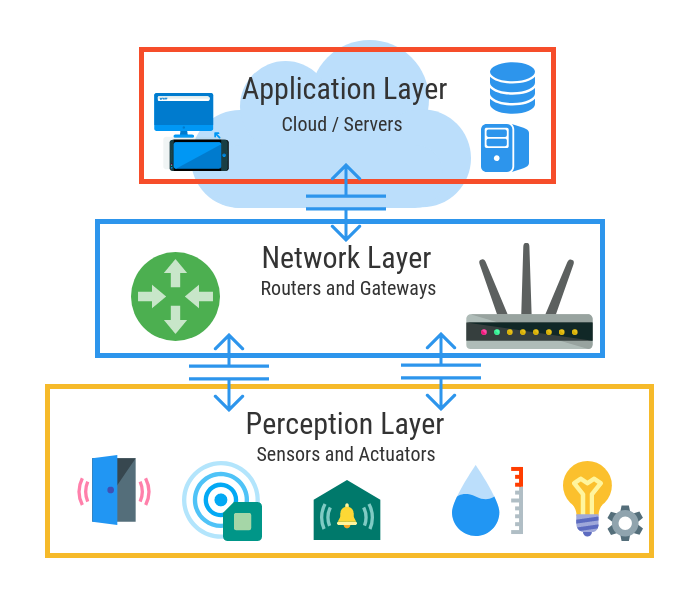
\includegraphics[width=\linewidth]{imagenes/arch-3-layer.png}
    \caption{Arquitectura de 3 capas. \cite{fig-3-layer-arch}}
    \label{fig:figure1}
\end{figure}

\begin{figure}[ht!]
    \centering
    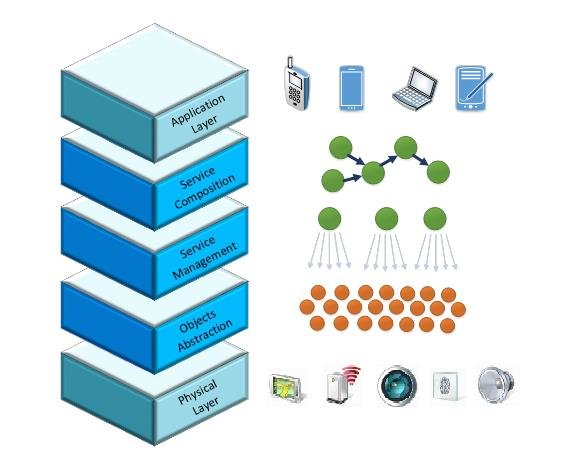
\includegraphics[width=\linewidth]{imagenes/SOA-based-architecture-for-IoT-middleware-1.jpg}
    \caption{Arquitectura de 4 capas. \cite{fig-4-layer-arch}}
    \label{fig:figure2}
\end{figure}


\subsection{Tecnologías asociadas}

Teniendo en cuenta las arquitecturas mencionadas anteriormente, el IoT cuenta con varias tecnologías que hacen posible la cumplir el objetivo de cada capa de la arquitectura. A continuación se comentan sobre las tecnologías que nos encontramos en la Arquitectura basada en SoA. \cite{lin2017survey}-\cite{tripathy2017internet}

\subsubsection{Capa de percepción}

En la capa de percepción, la función principal es identificar y rastrear objetos. Para lograr esta función, se pueden implementar las siguientes tecnologías pueden ser implementadas.

\begin{itemize}
    \item \textbf{Radio frequency identification (RFID)}. El sistema RFID se compone de uno o varios lectores y varias etiquetas RFID. Utiliza campos electromagnéticos de radiofrecuencia para enviar los datos adjuntos. Las etiquetas que se adjuntan a ella, almacenan datos electrónicamente que pueden ser leídos por RFID cuando se encuentra en la proximidad del lector. \cite{7589556}
    \item \textbf{Redes de sensores inalámbricos (WSN)}. Pueden desempeñar un papel muy importante en el IoT. Las WSN pueden monitorizar y rastrear el estado de los dispositivos, y transmitir los datos de estado al centro de control o a los nodos de enlace a través de múltiples saltos. Por lo tanto, las WSN pueden considerarse como un puente más entre el mundo real y el mundo cibernético. \cite{lin2017survey}
\end{itemize}

\subsubsection{Capa de red} \label{protocolos}

La capa de red se utiliza para determinar el enrutamiento y proporcionar soporte de transmisión de datos a través de redes heterogéneas integradas. A continuación, se presentan algunos protocolos que pueden permitir la comunicación fiable y segura en el IoT. \cite{lin2017survey}

\begin{itemize}
    \item \textbf{IEEE 802.15.4}. Se lanzó a principios de 2003 y ha satisfecho la necesidad de dispositivos de bajo consumo. Es un protocolo diseñado para la capa física y la capa MAC en redes inalámbricas de área personal (WPAN). El objetivo de IEEE 802.15.4 es centrarse en las WPAN de baja velocidad, proporcionando las conexiones de baja velocidad de todas las cosas en un área personal con bajo consumo de energía, baja tasa de transmisión, y bajo coste. Una de las tecnologías que rompen los esquemas es el estándar de radio IEEE 802.15.4. \cite{8320780}
    \item \textbf{6LoWPAN}. Las WPAN de baja potencia (LoWPAN) están organizadas por un gran número de dispositivos de bajo coste conectados mediante comunicaciones inalámbricas. En comparación con otros tipos de redes, las LoWPAN presentan una serie de ventajas, como el tamaño reducido de los paquetes, baja potencia, poco ancho de banda, etc. Como mejora, el protocolo 6LoWPAN fue diseñado combinando IPv6 y LoWPAN. En 6LoWPAN, los paquetes IPv6 pueden transmitirse a través de redes IEEE 802.15.4. Debido a que bajo coste y el bajo consumo de energía, 6LoWPAN es adecuado para el IoT, en el que se incluye un gran número de dispositivos de bajo coste.
    \item \textbf{ZigBee}. Es una tecnología de red inalámbrica, diseñada para la comunicación a corto plazo con bajo consumo de energía. En el protocolo ZigBee se incluyen cinco capas la capa física, la capa MAC, la capa de transmisión, la capa de capa de red y la capa de aplicación. Las ventajas de las redes ZigBee son el bajo consumo de energía, el bajo coste baja tasa de datos, baja complejidad, fiabilidad y seguridad.
    \item \textbf{Z-Wave}. Es una tecnología de comunicación inalámbrica a corto plazo con las ventajas de bajo coste, bajo consumo de energía consumo de energía y gran fiabilidad. El objetivo principal de Z-Wave es proporcionar una transmisión fiable entre una control y uno o más dispositivos finales, y Z-wave es adecuada para la red con poco ancho de banda. La red Z-wave soporta la tecnología de enrutamiento dinámico, y cada esclavo almacena una lista en su memoria, que es actualizada por el controlador. La principal diferencia entre ZigBee y Z-wave es la banda de frecuencia en la que opera la capa física.
    \item \textbf{Message Queue Telemetry Transport (MQTT)}. Usa la técnica de publicación/suscripción, es un protocolo de mensajería, que se utiliza para recoger datos medidos en sensores remotos y transmitir los datos a los servidores. MQTT es un protocolo simple y ligero, y soporta la red con bajo ancho de banda y alta latencia. MQTT puede implementarse en varias plataformas para conectar en Internet, y por lo tanto MQTT puede ser utilizado como un protocolo de mensajería entre sensores/actuadores y servidores, lo que hace que MQTT desempeñe un papel importante en el IoT.
    \item \textbf{Constrained Application Protocol (COAP)}. Es un protocolo de mensajería basado en la arquitectura de transferencia de estado representativa (REST). Dado que la mayoría de los dispositivos del IoT tienen recursos limitados (es decir, poco almacenamiento y poca capacidad de cálculo), HTTP no puede utilizarse en el IoT, debido a su complejidad. Para superar este problema, se propuso CoAP para modificar algunas funciones de HTTP con el fin de satisfacer los requisitos de el IoT. En términos generales, CoAP es el protocolo de la capa de aplicación en la pila de protocolos 6LoWPAN, y tiene como objetivo permitir que los dispositivos con recursos limitados logren interacciones RESTful. La comunicación de grupo y la notificación push son compatibles con CoAP, pero la difusión no lo es. La observación de recursos, el transporte de recursos en bloque descubrimiento de recursos, interacción con HTTP, y seguridad son todas las características importantes proporcionadas por CoAP.
    \item \textbf{Advanced Message Queuing Protocol (AMQP)}. Es un protocolo de colas de mensajes de estándar abierto que se utiliza para proporcionar servicios de mensajes (colas, enrutamiento, seguridad, fiabilidad, etc.) en la capa de aplicación. AMQP se centra en los entornos orientados a mensajes y puede considerarse como un protocolo middleware orientado a mensajes. Usando AMQP, los clientes pueden lograr una comunicación estable con los middlewares de mensajes, incluso si estos clientes y middlewares son producidos por diferentes lenguajes de programación.
    \item \textbf{Extensible Messaging and Presence Protocol (XMPP)}. Es un protocolo de mensajería instantánea basado en protocolos de transmisión XML. XMPP hereda las características del protocolo XML, por lo que XMPP tiene una gran escalabilidad, direccionamiento y capacidades de seguridad, y puede ser utilizado para el chat multipartito, voz y vídeo, y telepresencia. En XMPP, se incluyen los siguientes tres funciones: 1) cliente; 2) servidor; y 3) pasarela, así como así como la comunicación bidireccional entre dos partes de estos tres roles.
    \item \textbf{Data Distribution Service (DDS)}. Es un protocolo de publicación/suscripción para soportar la comunicación de dispositivo a dispositivo de alto rendimiento. DDS esta centrado en los datos, en el que se puede soportar la multidifusión para lograr una gran QoS y una alta fiabilidad. La arquitectura de publicación/suscripción sin intermediario hace que DDS sea adecuado para el IoT con restricciones de tiempo real y para la comunicación entre dispositivos.\cite{lin2017survey}
\end{itemize}

\subsubsection{Capa de servicio}

Como se ha descrito anteriormente, la capa de servicio se encuentra entre la capa de red y la capa de aplicación, y proporciona servicios eficientes y seguros a los objetos o aplicaciones. En la capa de servicio, deben incluirse las siguientes tecnologías habilitadoras para garantizar que el servicio pueda prestarse de forma eficiente: tecnología de interfaz, tecnología de gestión de servicios, tecnología de middleware y tecnología de gestión y compartición de recursos.

\begin{itemize}
    \item \textbf{Interfaz}. Debe diseñarse en la capa de servicio para garantizar el intercambio de información eficiente y seguro para las comunicaciones entre dispositivos y aplicaciones. Además, la interfaz debe gestionar eficientemente los dispositivos interconectados, incluyendo la conexión de dispositivos, la desconexión de dispositivos, la comunicación de dispositivos y el funcionamiento de dispositivos. Para dar soporte a las aplicaciones en el IoT, un perfil de interfaz (IFP) puede ser considerado como un estándar de servicio, que puede ser utilizado para facilitar las interacciones entre los servicios proporcionados por varios dispositivos o aplicaciones. Para lograr un IFP eficiente, debe implementarse el plug and play universal. Con el desarrollo del IoT, se han realizado varios esfuerzos sobre la interfaz.
    \item \textbf{Gestión de servicios}. Puede descubrir eficazmente los dispositivos y aplicaciones, y programar servicios eficientes y fiables para satisfacer las solicitudes. Un servicio puede considerarse como un comportamiento, que incluye la recogida, el intercambio y el almacenamiento de datos, o una asociación de estos comportamientos para lograr un objetivo especial. En el IoT, algunos requisitos pueden ser satisfechos por un solo servicio, mientras que otros deben ser satisfechos mediante la integración de múltiples servicios.
    \item \textbf{Middleware}. Es un software o servicio de programación que puede proporcionar una abstracción interpuesta entre las tecnologías de IoT y las aplicaciones. En el middleware se ocultan los detalles de las diferentes tecnologías y se proporcionan las interfaces estándar para que los desarrolladores puedan centrarse en el desarrollo de aplicaciones sin tener en cuenta la compatibilidad entre las aplicaciones y las infraestructuras. Así pues, mediante el uso de middleware, los dispositivos y las aplicaciones con diferentes interfaces pueden intercambiar información y compartir recursos entre sí. \cite{lin2017survey}
\end{itemize}


\subsection{Aplicaciones}

El IoT es una tecnología emergente que reclama la tercera posición después del ordenador e Internet. En esta tecnología, las cosas se conectan a Internet de una forma u otra, lo que da lugar a una enorme cantidad de datos que deben ser procesados, almacenados y representados de forma eficiente. Las aplicaciones de el IoT varían en diferentes campos e incluyen aplicaciones personales, industriales y nacionales. En los últimos años, estas aplicaciones han aumentado constantemente y algunas de ellas ya están desplegadas y se utilizan a diferentes niveles. Las aplicaciones de IoT requieren hardware, middleware y presentación. Estas aplicaciones tienen características como la comunicación de dispositivos con el mundo real, interacción con el entorno interacción entre personas y dispositivos, tareas rutinarias automáticas con menos supervisión, infraestructura organizada y seguridad en la comunicación.\\

Son muchas las aplicaciones que se están desarrollando hoy en día y en los últimos años las aplicaciones de IoT han ido a más. Las aplicaciones requieren un avance RFID y tecnologías de direccionamiento, con mejor visualización y capacidad de almacenamiento. Teniendo en cuenta los requisitos de IoT se ha desarrollado una arquitectura de aplicaciones para un menor consumo de energía. Algunos ejemplos que nos encontramos de aplicaciones del IoT son: \cite{8320780}-\cite{tripathy2017internet}

\begin{itemize}
    \item \textbf{Casas inteligentes}. En este caso nos encontramos nuevos inventos que se conectan y controlan nuestros hogares desde nuestros teléfonos.
    \item \textbf{Wearable Technology}. Se han diseñado e implementado varios productos diseñados y aplicados en este ámbito, desde anillos a calzado, y desde relojes hasta mochilas. Esta tecnología puede verse en todas partes.
    \item \textbf{Ciudades inteligentes}. Es un área de tecnología al servicio de las personas, y esta tecnología se construye esencialmente en torno al usuario. Una ciudad no es más que una red diseñada para optimizar los recursos.
    \item \textbf{Red inteligente}. Desde que las instalaciones del IoT se han añadido a la red anterior de datos, se han vuelto más inteligentes, lo que significa más y más información de la red. Desde que el IoT ha ayudado a convertirse en el sistema de suministro de energía de dos maneras la información se enviará al centro principal sobre el uso y el consumo.
    \item \textbf{Atención sanitaria inteligente}. Es un elemento vital para nuestra salud y bienestar, ya sea para el hospital, la odontología o la residencia de ancianos. Este apunta a todos los grupos de edad de la población al mismo tiempo. Para ello se requiere eficacia y menos costes.
\end{itemize}

\subsection{Retos}

Muchas empresas se apresuran a crear aplicaciones para el IoT y gastan enormes sumas de dinero porque es la próxima gran oportunidad. Se han introducido lavadoras, sistemas de calefacción y frigoríficos inteligentes. El IoT ha traído muchos cambios y dimensiones positivas. Sin embargo, tienen una serie de riesgos y desafíos. \cite{8320780}-\cite{tripathy2017internet}

\begin{itemize}
    \item \textbf{Seguridad y privacidad}. Las aplicaciones del IoT y las áreas inteligentes manejan muchos datos a diario y estos datos se comparten entre dispositivos. La información sobre casas, edificios y coches se comparte entre dispositivos todo el tiempo. Toda esta información exige un mejor sistema de gestión. Los sistemas de seguridad existentes no son adecuados en muchos aspectos y pueden causar graves problemas al usuario. Un error puede hacer que la seguridad del hogar, los coches, los edificios y los datos guardados sean vulnerables.
    \item \textbf{Comunicación fiable}. El IoT se compone de tecnologías fijas y móviles, y se intenta conseguir una comunicación bidireccional sin pérdida de datos y con total fiabilidad.
    \item \textbf{Consumo de energía}. Los dispositivos deben ser capaces de comunicarse con un menor uso de la batería porque estos dispositivos se despliegan lejos y necesitan funcionar con baterías.
    \item \textbf{Interoperabilidad}. Este requiere que los dispositivos se comuniquen entre sí. A nivel de usuario, el usuario puede tener múltiples dispositivos que funcionen en múltiples plataformas. El usuario no querrá quedarse con un solo dispositivo. En cambio, un usuario puede querer diversidad en caso de elegir un dispositivo.
\end{itemize}


\section{Seguridad}

Durante las primeras décadas de su existencia, las redes informáticas eran utilizadas principalmente por los investigadores universitarios para enviar correos electrónicos y por los empleados de las empresas para compartir impresoras. En estas condiciones, la seguridad no recibía mucha atención. Pero ahora, cuando millones de ciudadanos de a pie utilizan las redes para realizar operaciones bancarias, comprar y presentar sus declaraciones de impuestos, y se han encontrado puntos débiles tras puntos débiles, la seguridad de las redes se ha convertido en un problema de proporciones masivas. \\ 

La seguridad, trata de asegurar que los entrometidos no puedan leer, o peor aún, modificar secretamente los mensajes destinados a otros destinatarios. Se trata de que las personas intenten acceder a servicios remotos para los que no están autorizadas. La seguridad también se ocupa de los problemas de los mensajes legítimos que son capturados y reproducidos, y de las personas que más tarde intentan negar haber enviado ciertos mensajes. La mayoría de los problemas de seguridad son causados intencionadamente por personas malintencionadas que intentan obtener algún beneficio, llamar la atención o perjudicar a alguien. \\ \cite{Tanenbaum2011ComputerN5}

\subsection{Características de seguridad en el IoT}

Este trabajo al estar relacionado con el IoT nos centramos en analizar la seguridad relacionada con este. Podemos analizar distintos aspectos de la seguridad, como puede ser en la transmisión de datos, hardware, software, pero todos estos puntos tienen una serie de puntos en común:

\begin{itemize}
    \item  \textbf{Confidencialidad}. La confidencialidad puede garantizar que los datos sólo estén disponibles para los usuarios autorizados durante todo el proceso, y que no puedan ser escuchados o interferidos por usuarios no autorizados. En IoT, la confidencialidad es un principio de seguridad importante, ya que un gran número de dispositivos de medición (RFID, sensores, etc.) pueden integrarse en IoT. Por lo tanto, es fundamental garantizar que los datos recogidos por un dispositivo de medición no revelen información segura a sus dispositivos vecinos. Para lograr una gran confidencialidad, deben mejorarse las técnicas, incluyendo mecanismos seguros de gestión de claves.
    \item  \textbf{Integridad}. La integridad puede garantizar que los datos no puedan ser manipulados por interferencias intencionadas o no intencionadas durante la entrega de datos en las redes de comunicación, proporcionando en última instancia los datos precisos para los usuarios autorizados. La integridad es importante para IoT, porque si las aplicaciones de IoT reciben datos falsificados o manipulados, se puede estimar un estado de funcionamiento erróneo y se pueden realizar comandos de retroalimentación equivocados, lo que podría interrumpir aún más el funcionamiento de las aplicaciones de IoT. Para lograr una integridad aceptable, deben desarrollarse y aplicarse mecanismos de integridad de datos seguros mejorados y aplicarlos.
    \item \textbf{Disponibilidad}. La disponibilidad puede garantizar que los datos y los dispositivos estén disponibles para los usuarios y servicios autorizados siempre que se soliciten los datos y los dispositivos. En IoT, los servicios suelen solicitarse en tiempo real, y los servicios no pueden programarse y prestarse si los datos solicitados no pueden entregarse a tiempo. Por lo tanto, la disponibilidad es también un importante principio de seguridad. Una de las amenazas más graves para la disponibilidad es el ataque de denegación de servicio (DoS), y las técnicas mejoradas, protocolos de enrutamiento seguros y eficientes, para garantizar la disponibilidad en el IoT. \cite{lin2017survey}

\end{itemize}


\subsection{Aspectos legales y éticos}

La seguridad es un requisito importante en el diseño y desarrollo para un proyecto, por ello hay que considerar los aspectos normativos, en especial relacionados con la privacidad, ya que es esencial en el desarrollo de sistemas TIC`s. \\

Se va a destacar la \textbf{Agencia Española de Protección de Datos}, que en 2014 realizaron el primer dictamen relacionado con el IoT. \\

En el \textbf{Dictamen 8/2014} del Grupo de Trabajo del Artículo 29, ahora Comité Europeo de Protección de Datos, se define IoT como aquella infraestructura en la que múltiples sensores incorporados a dispositivos comunes y cotidianos registran, someten a tratamiento, almacenan y transfieren datos e interactúan con otros dispositivos o sistemas haciendo uso de sus capacidades de conexión en red. En muchos casos, dichos objetos están asociados a identificadores únicos y tratan datos personales. \\

El Grupo de trabajo del artículo 29 decidió emitir este Dictamen por considerar que el IoT plantea
diversos retos importantes relativos a la intimidad y la protección de los datos, algunos nuevos, otros
más tradicionales, pero amplificados por el aumento exponencial del tratamiento de datos que conlleva
la evolución de este fenómeno. La importancia de la aplicación del marco jurídico de protección de los
datos de la UE y las correspondientes recomendaciones que se presentan más abajo se deben
contemplar a la luz de estos retos. \cite{aepd-info} \\

Uno de los puntos que se puede destacar es que para que los usuarios del Internet de las Cosas puedan permanecer siempre en control de sus datos deben saber claramente cómo y para qué se van a utilizar los mismos. Deben dar su consentimiento expreso tras recibir la información de forma clara y transparente. \\

Relativo al proyecto, hay que tener en cuenta secciones como la de \textbf{Creadores de aplicaciones} que dice lo siguiente \cite{dictamen8-24}:

\begin{itemize}
    \item \textit{``Se deben elaborar avisos o advertencias para recordar frecuentemente a los usuarios que los sensores están recogiendo datos. Si el creador de la aplicación no tiene acceso directo al dispositivo, la aplicación debe enviar periódicamente al usuario una notificación para recordarle que sigue registrando datos. ``}
    \item \textit{``Las aplicaciones deben facilitar el ejercicio del derecho del interesado al acceso, la modificación y la eliminación de la información personal recogida por los dispositivos de IO. ``}
    \item \textit{``Los creadores de aplicaciones deben proporcionar herramientas para que los interesados exporten tanto los datos primarios como los agregados en un formato normalizado y fácil de utilizar. ``}
    \item \textit{``Los creadores deben prestar una atención especial a los tipos de datos que se someten a tratamiento y a la posibilidad de deducir de ellos datos personales sensibles. ``}
    \item \textit{``Los creadores de aplicaciones deben aplicar el principio de minimización de datos. Cuando los fines se puedan alcanzar mediante datos agregados, los creadores no deberán acceder a los datos primarios. De manera más general, los creadores deben seguir un enfoque de intimidad desde el diseño y reducir la cantidad de datos recogidos al mínimo necesario para la prestación del servicio. ``}
\end{itemize}

Como conclusión de este dictamen obtenemos que, los tratamientos basados en IoT precisan de modelos que incorporen los requisitos normativos, estándares y mecanismos de certificación para garantizar un nivel de protección de derechos y libertades de las personas. Pudiendo ser utilizados por las personas sin amplios conocimientos con la confianza de que no se vulnerará su privacidad. \cite{aepd-info}


}